\documentclass[11pt]{article}
\usepackage{amsmath}
\usepackage{amssymb}
\usepackage{graphicx}
\usepackage{fancyhdr}
\usepackage{enumerate}
\usepackage{titlesec}
\usepackage[colorlinks=true,urlcolor=blue]{hyperref}

\titlespacing{\subsubsection}{0pt}{0pt}{0pt}

% No page numbers
%\pagenumbering{gobble}
\newenvironment{code}{\fontfamily{pcr}\selectfont} {\par}

% MARGINS (DO NOT EDIT) ---------------------------------------------
\oddsidemargin  0.25in \evensidemargin 0.25in \topmargin -0.5in
\headheight 0.2in \headsep 0.1in
\textwidth  6.5in \textheight 9in
\parskip 1.25ex  \parindent 0ex \footskip 20pt
% ---------------------------------------------------------------------------------

% HEADER (DO NOT EDIT) -----------------------------------------------
\newcommand{\problemnumber}{0}
\newcommand{\myname}{name}
\newfont{\myfont}{cmssbx10 scaled 1000}
\pagestyle{fancy}
\fancyhead[L]{\myfont Question \problemnumber, Problem Set 1, CS229}
\fancyhead[R]{John Mern, jmern91@stanford.edu}
\newcommand{\newquestion}[1]{
\clearpage % page break and flush floats
\renewcommand{\problemnumber}{#1} % set problem number for header
\phantom{}  % Put something on the page so it shows
}
% ---------------------------------------------------------------------------------


% BEGIN HOMEWORK HERE
\begin{document}

% Question 1
\newquestion{1(a)}
The algorithm converged in about 30,0000 iterations for dataset A, however, it did not converge in over 3M iterations for set B. 

\newquestion{1(b)}

As can be seen below, the gradient of A quickly converges to it's asymptotic limit of zero. The gradient for B, however, remains non-zero as the gradient decay rate flattens. 

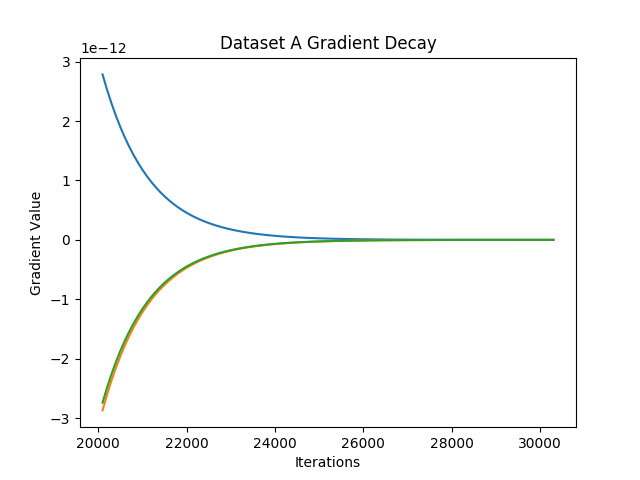
\includegraphics[scale=0.4]{P1b_1.png}
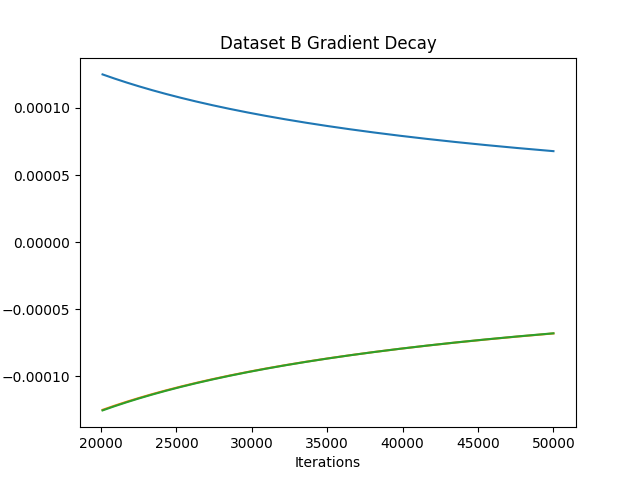
\includegraphics[scale=0.4]{P1b_2.png}

This is likely due to the fact that, while dataset A has no clear margin between the positive and negative examples, dataset B is almost perfectly separable. For a set that is nearly perfectly separable, the gradient becomes exteremely small for values near the optimal solution, causing the update step to decay rapidly. This prevents the gradient descent approach from converging. 

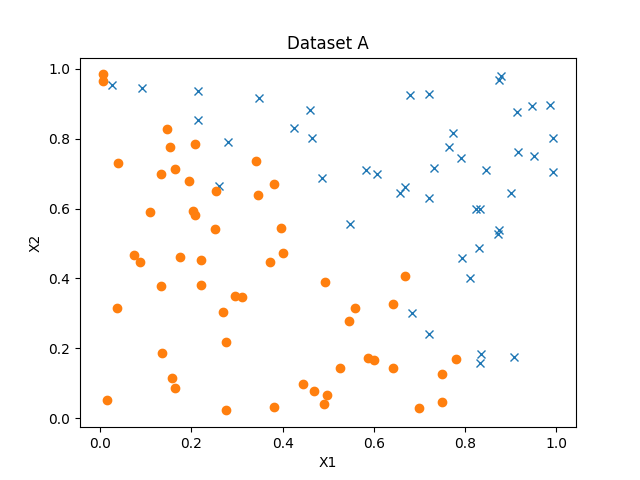
\includegraphics[scale=0.4]{P1b_3.png}
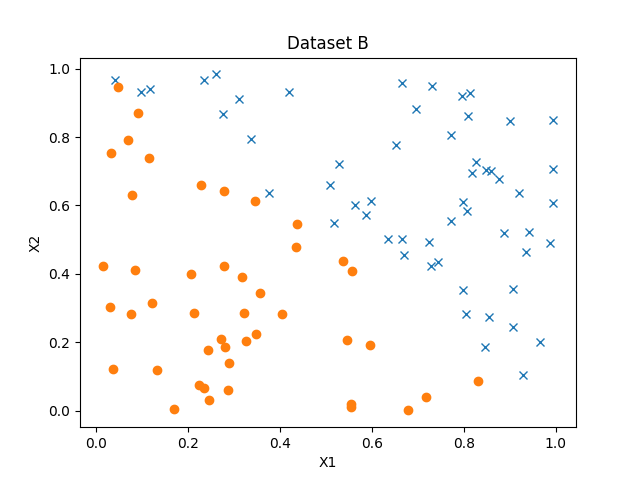
\includegraphics[scale=0.4]{P1b_4.png}

By removing the points that cause the non-zero margin in A, we get the resulting dataset shown below. Running the regression on this does not converge after 500K iterations. 

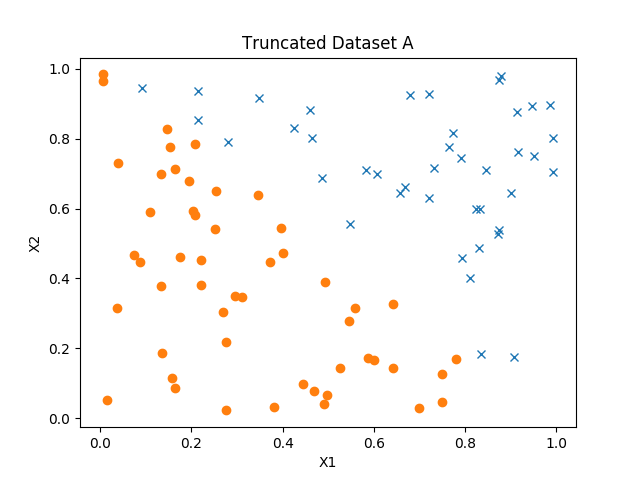
\includegraphics[scale=0.4]{P1b_5.png}

\newquestion{1(c)}

i. This will not aid significantly in convergence of separable sets. The gradient signal will still approach zero asymptotically as in B, and changing the learning rate will not change this trend. 

ii. This will not aid either. The graident does no rapidly change signs and is smooth and monotonic across the learning. Decreasing the learning rate will only further slow down the learning process. 

iii. This should aid in convergence. L2 regularization causes weights to tend toward small values. Smaller values of theta should help keep the value of the gradient larger as it decreases the denominator in the gradient term. 

iv. This would not help. The features are already of similar dimension.

v. This should help by causing more points to cross the optimal hyperplane, increasing the strength of the gradient signal.  

\newquestion{1(d)}

SVMs seek to maximize the margin between the separating hyperplane and the supporting hyperplane of each set. If using a hinge-loss with fixed margin, perfectly separable cases can be dealt with by ensuring a sufficiently large margin. 

\newquestion{1 (code)}

\begin{code}
\begin{verbatim}
import numpy as np 
import matplotlib.pyplot as plt

from lr_debug import * 

import pdb



def logistic_regression(X, Y, ints):
    m, n = X.shape
    theta = np.zeros(n)
    learning_rate = 10

    i = 0
    I = []
    Grad = []
    while True:
        i += 1
        prev_theta = theta
        grad = calc_grad(X, Y, theta)
        theta = theta  - learning_rate * (grad)
        if i % 100 == 0:
        	Grad.append(grad)
        	I.append(i)
        if i % 10000 == 0:
            print('Finished %d iterations' % i)
        if np.linalg.norm(prev_theta - theta) < 1e-15:
            print('Converged in %d iterations' % i)
            break
        if i >= ints:
        	print('Did not converge')
        	break
    return Grad, I

Xa, Ya = load_data('data_a.txt')
Xb, Yb = load_data('data_b.txt')

Xa_p = Xa[Ya>0, :]
Xa_n = Xa[Ya<0, :]

Xb_p = Xb[Yb>0, :]
Xb_n = Xb[Yb<0, :] 

gradA, IA = logistic_regression(Xa, Ya, 50000)

gradB, IB = logistic_regression(Xb, Yb, 50000)

gradA = np.array(gradA)
plt.figure()
plt.plot(IA[200:], gradA[200:,0])
plt.plot(IA[200:], gradA[200:,1])
plt.plot(IA[200:], gradA[200:,2])
plt.title('Dataset A Gradient Decay')
plt.xlabel('Iterations')
plt.ylabel('Gradient Value')
plt.show()

gradB = np.array(gradB)
plt.figure()
plt.plot(IB[200:], gradB[200:,0])
plt.plot(IB[200:], gradB[200:,1])
plt.plot(IB[200:], gradB[200:,2])
plt.title('Dataset B Gradient Decay')
plt.xlabel('Iterations')
plt.ylabel('Gradient Value')
plt.show()

plt.figure()
plt.plot(Xa_p[:,1], Xa_p[:,2], 'x')
plt.plot(Xa_n[:,1], Xa_n[:,2], 'o')
plt.title('Dataset A')
plt.xlabel('X1')
plt.ylabel('X2')
plt.show()

plt.figure()
plt.plot(Xb_p[:,1], Xb_p[:,2], 'x')
plt.plot(Xb_n[:,1], Xb_n[:,2], 'o')
plt.title('Dataset B')
plt.xlabel('X1')
plt.ylabel('X2')
plt.show()

Xap_ = []
Yap_ = []

for i in range(Xa_p.shape[0]):
	if 1 - Xa_p[i,1] <= Xa_p[i,2]:
		Xap_.append(Xa_p[i,:])
		Yap_.append(1)

Xap_ = np.array(Xap_)
Yap_ = np.array(Yap_)

Xan_ = []
Yan_ = []

for i in range(Xa_n.shape[0]):
	if 1 - Xa_n[i,1] >= Xa_n[i,2]:
		Xan_.append(Xa_n[i,:])
		Yan_.append(-1)

Xan_ = np.array(Xan_)
Yan_ = np.array(Yan_)
plt.figure()
plt.plot(Xap_[:,1], Xap_[:,2], 'x')
plt.plot(Xan_[:,1], Xan_[:,2], 'o')
plt.title('Truncated Dataset A')
plt.xlabel('X1')
plt.ylabel('X2')
plt.show()

Xa_ = np.vstack([Xap_, Xan_])
Ya_ = np.vstack([Yap_.reshape([-1,1]), Yan_.reshape([-1,1])]).squeeze()
grad_, I_ = logistic_regression(Xa_, Ya_, 500000)
\end{verbatim}
\end{code}

\newquestion{2(a)}




\end{document}
